\documentclass[11pt]{article}
\usepackage[utf8]{inputenc}
\usepackage[english]{babel}
\usepackage{amssymb,amsmath,amsthm,mathtools}
\usepackage{enumitem, graphicx, hyperref}

\topmargin -0.5in
\textheight 9.0in
\oddsidemargin  -0.05in
\evensidemargin -0.05in
\textwidth 6.5in
\renewcommand
\baselinestretch{1.0}

\newtheorem{theorem}{Theorem}[section]
\newtheorem{corollary}{Corollary}[theorem]
\newtheorem{lemma}[theorem]{Lemma}
\newtheorem{definition}{Definition}[section]
\newtheorem*{remark}{Remark}

\allowdisplaybreaks
\numberwithin{equation}{section}
 
\newcommand{\tr}{{\text{tr}}}
\newcommand{\B}[1]{\textbf{#1}}
\newcommand{\T}[1]{\texttt{#1}}

\title{QBist Bell Inequalities}
\author{Matthew B. Weiss}
\date{\today}

\begin{document}
\maketitle 

\begin{abstract}
In this short note, we reinterpret violations of Bell inequalities as imposing lower bounds on the distance between the QBist Born matrix and the identity: a nonzero bound implies that the Born Rule diverges from the law of total probability. The value of the bound itself may be regarded as a quantifying the nonclassicality of the Bell scenario as captured by a QBist reference device. In particular, we show that 
\begin{equation*}
	\lVert \Phi- I\rVert_F \ge 	\frac{\Delta}{\sigma_{\max}(\B{T})\lVert \B{c}\rVert_2}.
\end{equation*}
Here we've assigned QBist reference devices to each party, and $\Phi$ is the Born matrix for the composite reference device. $\Delta$ is the numerical violation of the particular Bell inequality considered, $\B{T}$ is a matrix encoding the reference probabilities which characterize the initial entangled state shared by the parties as well as the possible measurements each party may perform. Finally, $\B{c}$ encodes the linear functional determining the Bell observable. $\lVert \cdot \rVert_F$ is the Frobenius norm, $\sigma_{\max}$ is the maximal singular value, and $\lVert \cdot \rVert_2$ is the Euclidean norm. The form of the expression can be easily generalized to other choices of norms. 
\end{abstract}

\section{A variation on the double slit experiment}

We begin by briefly reviewing the QBist reference device formalism. Fixing a Hilbert space dimension $d$, we call a \emph{reference device} a device which first performs an informationally complete (IC) measurement $\{R_i\}$ and then prepares one of a set of informationally complete states $\{\sigma_i\}$. Informational-completeness means that the POVM elements (states, resp.) span the space of operators on $\mathcal{H}_d$: it follows that the reference measurement suffices to characterize any arbitrary state, and the reference states suffice to characterize any arbitrary measurement. 

In particular, by means of an IC reference device, the Born rule can  be re-expressed as a consistency condition on an agent's probability assignments across several experiments. To see this, consider first preparing a quantum system according to $\rho$. We then send the system into a reference device $\{R_i, \sigma_i\}$ that can be turned \emph{on} or \emph{off}. Subsequently, the system is sent into an arbitrary measurement apparatus $\{E_j\}$. This is in analogy to the double slit experiment where the final measurement would be a detection of a particle against the back wall, and the intermediate measurement would be a which-slit detection. The novelty is that we now consider the intermediate measurement to be informationally complete.
\begin{center}
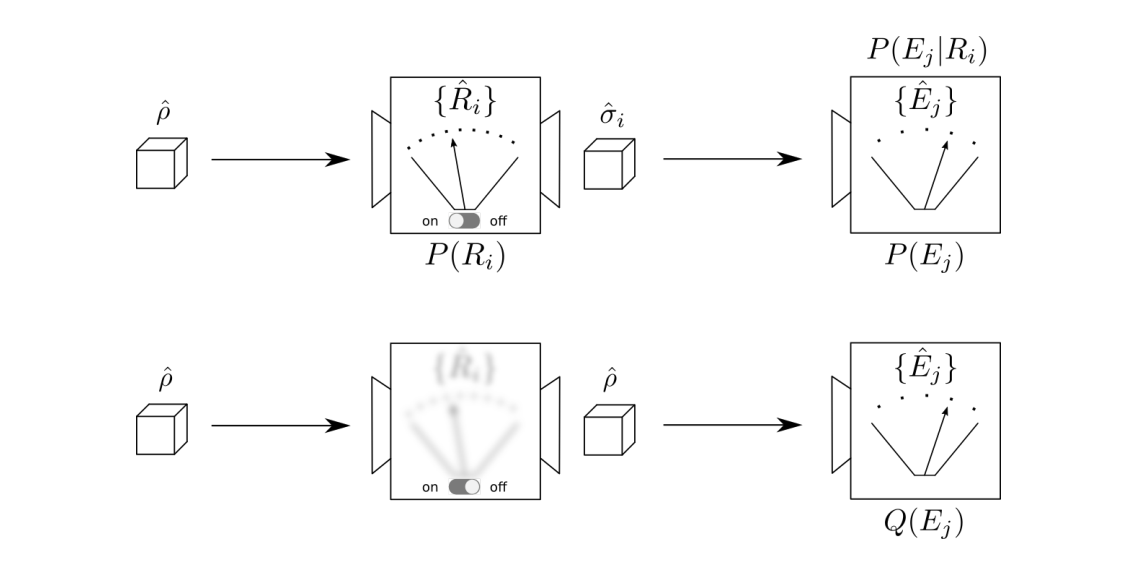
\includegraphics[scale=0.8]{img/sky_ground}	
\end{center}
In the first case, it is not hard to show that one's probability assignments ought to be related by the law of total probability (LTP),
\begin{align}
P(E_j)&=\sum_i P(E_j|R_i)P(R_i)	.
\end{align}
In the second case, when the reference device is turned \emph{off}, the Born rule tells us that we ought to assign
\begin{align}
Q(E_j)	&= \tr(E_j\rho).
\end{align}
By informational-completeness, however, a density matrix $\rho$ is equivalent to probability assignments $P(R_i)=\tr(R_i\rho)$, and a POVM element $E_j$ is equivalent to the assignment of probabilities $P(E_j|R_i)=\tr(E_j\sigma_j)$. Therefore we ought to be able to calculate $Q(E_j)$ directly in terms of these reference probabilities instead of using POVM elements and density matrices. Let us see how this can be done in the simplest case.

If the number of reference outcomes is $d^2$, the corresponding POVM elements must in fact form a linearly independent basis for the operator space. Let $|A)$ denote the vectorization of the matrix $A$, and recall that $\tr(B^\dagger A)= (B|A)$. Let $\B{R}_{ij}=(R_i|j)$ be the matrix whose rows are $(R_i|$ and and $\B{S}_{ij}=(i|S_j)$ be the matrix whose columns are $|\sigma_i)$. These are both $d^2 \times d^2$ matrices and by informational-completeness, $\B{R}$ and $\B{S}$  will in fact be invertible. Thus
\begin{align}
	Q(E_j)&=(E_j|\rho)=(E_j|\B{S}\B{S}^{-1}\B{R}^{-1}\B{R}|\rho)=(E_j|\B{S}(\B{RS})^{-1}\B{R}|\rho).
\end{align}
To interpret this expression, we note that $(E_j|\B{S}$ is the row vector of conditional probabilities $P(E_j|R_i)$; that $\B{R}|\rho)$ is the column vector of probabilities $P(R_i)$; and that $\B{RS}$ is the matrix of conditional probabilities $P(R_i|R_j)$, for getting a reference outcome, given a reference preparation. Calling $\Phi \equiv (\B{RS})^{-1}$ the \emph{Born matrix}, we've thus shown that
\begin{align}
\label{Born_rule}
Q(E_j)=\sum_{ik} P(E_j|R_i)\Phi_{ik}P(R_k).
\end{align}
In this way, the Born rule appears as a \emph{deformation of the law of total probability} by the Born matrix $\Phi$. Crucially, everything in Eq.\! \ref{Born_rule} is grounded in a probability assignment, even $\Phi$, which is the inverse of a conditional probability matrix. 


In \cite{PhysRevResearch.2.013074}, the authors introduced  $||\Phi-I||$  with respect to any unitarily invariant norm as a measure of the LTP deformation and proved that among all reference devices with $d^2$ outcomes,  $||\Phi-I||$ attains its minimum if and only if the reference measurement is a SIC-POVM and the reference states are proportional to POVM elements, $\sigma_i = R_i/\tr(R_i)$ (an assumption we will generally make throughout). A SIC is defined as a set of $d^2$ rank-1 projectors $\{\sigma_i\}$ satisfying $\tr(\sigma_i \sigma_j)=\frac{d\delta_{ij}+1}{d+1}$; rescaling the $\sigma_i$'s by $\frac{1}{d}$ yields POVM elements. It directly follows that the expression for the Born rule simplifies to
\begin{align}
Q(E_j)=\sum_i P(E_j|R_i)\left[(d+1)P(R_i)-\frac{1}{d}\right]	,
\end{align}
and the value $||\Phi-I||$ in this case may be regarded as the measure of the irreducible nonclassicality of quantum theory itself. The intuition is that classically, an informationally complete reference measurement would be, for example, to read off the positions and momenta of all the particles in a system in a non-disturbing way. The particles ``really have'' positions and momenta, and so whether or not one actually performs the reference measurement, one ought to use the law of total probability to calculate probabilities for any other observable. So in classical theory, it is always possible to pick a reference device such that $\Phi=I$: but this is precisely \emph{forbidden} by quantum theory. The closest one can get is to take $\Phi_{\text{SIC}} = (d+1)I -\frac{1}{d}J$, where $J$ is the matrix of all 1's. 

 This is suggestive of the idea that quantum systems don't ``really have'' underlying properties which are read off by  measurements, even reference measurements, but that, as QBism holds, the outcomes of measurement are better regarded as the possible consequences for an individual agent gambling upon a nature which is being continually co-created. But for a single system, this is heuristic and not at all a proof: after all, the outcomes of any single-system quantum experiment can be spoofed by a laptop computer which is generally regarded to operate on definite properties by perfectly definite rules. From this point of view, there is nothing to exclude the hypothesis that a single quantum system has some definite, yet unknown properties which are however disturbed by measurement. The situation is different, however, when we consider multipartite scenarios. There the violation of Bell's inequalities force us into a quandary: either quantum systems have underlying properties that condition the results of measurement, but these properties may be disturbed \emph{without regard for locality};  or else the outcomes of measurements are created in the act of measurement for the individual observer. (We exclude here the evasion of the quandary by the hypothesis of a multiverse.) Arguably, if we truly understood \emph{why the Born rule} at the deepest possible level, the difference between single and multipartite scenarios would appear less decisive: one imagines the force of a full derivation of the Born rule being so powerful that afterwards one could hardly contemplate any other form of reasoning about events and probabilities, so that in its light all concerns about e.g., Bell local models would be seen as atavistic, throwbacks to a time before complete clarity on the message of quantum theory. In the meantime, however, it would be to our benefit to directly connect violations of the LTP as quantified by  $\lVert  \Phi - I\rVert$ to violations of Bell inequalities and thus to evidence against so-called \emph{local realism}.

\section{Bell polytopes}

Consider a multipartite scenario, where $n$ distant parties share an entangled quantum system, and each party agrees to choose from a menu of potential measurements on the part local to them. In the simplest case, suppose Alice has a choice of measurements $\{A_i\}$ each of which has outcomes $\{a_i\}$, and Bob has a choice of measurements $\{B_i\}$ each of which has outcomes $\{b_i\}$. We can then consider the joint probability distribution $P(a_i, b_j|A_k, B_l)$. In particular, following Bell, we may consider the subset of all joint probability distributions which can be expressed
\begin{align}
P(a_i, b_j|A_k, B_l) = \sum_m P(a_i|A_k, \lambda_m)P(b_j|B_l, \lambda_m)P(\lambda_m),	
\end{align}
where $P(\lambda_m)$ is a distribution over some underlying ``hidden variables'' $\{\lambda_m\}$, while $P(a_i|A_k, \lambda_m)$ and $ P(b_j|B_l, \lambda_m)$ are response functions which depend only upon Alice (or Bob's, respectively) local choice of measurement---and the hidden variables. The point is that, for Bell, any correlations in Alice and Bob's measurement outcomes ought to be explained by correlations between the hidden variables which the quantum systems are supposed to have agreed upon before they were separated. The set of all such ``classical'' joint probability distributions for a given multipartite scenario forms a so-called \emph{Bell polytope} $\mathcal{L}$ \cite{Werner2001, Pironio2014}. 

For sake of intuition, consider for example the CHSH scenario. This is a bipartite scenario in which Alice and Bob each have a choice of two possible measurements, each of which has outcomes in $\{\pm 1\}$. Supposing that $P(a_i, b_j|A_k, B_l)$ takes the Bell form, one may derive the famous inequality
\begin{align}
-2 \leq \langle A_0 B_0\rangle + \langle A_0 B_1\rangle + \langle A_1B_0\rangle - \langle A_1 B_1\rangle  \leq 2.
\end{align}
Since $\langle A_k B_l\rangle = \sum_{ij} a_i b_j P(a_i, b_j|A_k, B_l)$,  letting
\begin{align}
s=\begin{pmatrix} 1 & 1 \\ 1 & -1 \end{pmatrix}	&& c_{ijkl}= a_i b_j s_{kl},
\end{align}
and denoting by $\B{p}$ and  $\B{c}$ the tensors $P(a_i, b_j|A_k, B_l)$ and $c_{ijkl}$ flattened into vectors, we may rewrite the CHSH inequality as
\begin{align}
-2 \leq \B{c}^T\B{p} \leq 2.
\end{align}
Note that $\B{p}$ is often called a \emph{behavior}. This is quite general: a Bell inequality always takes the form
\begin{align}
\B{c}^T\B{p}\leq \beta,	
\end{align}
where $\B{c}$ represents a particular observable, a linear functional acting on the joint probability vector, and $\beta$ is a classical bound derived by supposing that $\B{p}$ takes Bell form. Geometrically speaking, each Bell inequality $(\B{c}, \beta)$ defines a halfspace: their collective intersection is the Bell polytope $\mathcal{L}$.

Of course, quantum mechanics generally violates Bell inequalities. In the CHSH scenario, let  $A_0=Z, A_1=X$, and $B_0=(Z+X)/\sqrt{2}, B_1=(Z-X)/\sqrt{2}$, and let the initial state be $\rho=|\psi\rangle\langle \psi|$ where $|\psi\rangle=(|00\rangle+|11\rangle)/\sqrt{2}$. Then by the Born rule
\begin{align}
	P(a_i, b_j|A_k, B_l)=\tr\Big((\Pi_{a_i|A_k}\otimes \Pi_{b_j|B_l})\rho\Big), 
\end{align}
where $\Pi_{a_i|A_k}$ is the rank-1 projector onto the $a_i$ outcome of observable $A_k$. Famously, this choice of state and observables leads to $|\B{c}^T\B{p}|=2\sqrt{2}$, the maximal violation compatible with quantum mechanics. Let $(\B{c}, \beta)$ denote a Bell inequality which is violated. Then $\B{c}^T\B{p}=\beta + \Delta$ for $\Delta \ge 0$. It turns out we can bound the distance (with respect to a choice of norm $\lVert \cdot \rVert$) of the joint distribution $\B{p}$ to the Bell polytope $\mathcal{L}$ by
\begin{align}
\label{polytope_inequality}
\text{dist}(\B{p}, \mathcal{L})\ge \frac{\Delta}{\lVert \B{c}\rVert_*}	,
\end{align}
where $\lVert \cdot \rVert_*$ is the dual norm of $\lVert \cdot \rVert$. In particular, for a $p$-norm, $\lVert \B{x}\rVert_p = \left(\sum_i x_i^p\right)^{1/p}$, the dual norm is the H\"older dual $\lVert \B{x} \rVert_q$ satisfying $1/p + 1/q=1$ \cite{Boyd2004}: notice that that Euclidean norm is self-dual in this sense. As proven in Appendix \ref{duals}, the distance from  $\B{p}$ to the hyperplane $H=\{\B{x}|\B{c}^T\B{x}=\beta \}$ is $ \text{dist}(\B{p}, H)=\frac{\Delta}{\lVert \B{c}\rVert_*}$. Every (tight) Bell inequality defines a supporting hyperplane (the entire polytope lies in the corresponding half-space $\{\B{x}|\B{c}^T\B{x}\leq \beta\}$, and at least one vertex of the polytope lies on the hyperplane, or facet). Since the Bell polytope $\mathcal{L}$ lies entirely on the hyperplane's inner side, the distance to the hyperplane gives a lower bound on the distance to the whole polytope: $\text{dist}(\B{p}, \mathcal{L})\ge \text{dist}(\B{p}, H)=\frac{\Delta}{\lVert \B{c}\rVert_*}$.

\section{Bounding $\lVert \Phi -I \rVert$}

Fixing a multipartite Bell scenario, we may introduce a multipartite reference device: by the principle of local tomography, this can be done by choosing a reference device for each party. For example, in the CHSH scenario, we might suppose that Alice and Bob each have a qubit SIC reference measurement $\{R_i\}$, so that the overall reference measurement is $\{R_i \otimes R_j\}$. We can then characterize the quantum state of their two qubits with the joint probability distribution
\begin{align}
P(R_i, R_j)=\tr\Big((R_i\otimes R_j)\rho\Big),	
\end{align}
and characterize their measurements with
\begin{align}
P(a_i|A_k, R_u)=\tr(\Pi_{a_i|A_k}\sigma_u) && P(b_j|B_l, R_v)=\tr(\Pi_{b_j|B_l}\sigma_v),
\end{align}
where $\sigma_u = R_u/\tr(R_u)$. If $\Phi$ is the Born matrix for a single system reference device $\{R_i\}$, then Born matrix of the composite reference device $\{R_i \otimes R_j\}$ is just $\Phi \otimes \Phi$. Along the same lines as Eq. \! \ref{Born_rule}, we may then reexpress the joint probability distribution $P(a_i, b_j|A_k, B_l)$ in terms of reference probabilities,
\begin{align}
\label{composite_born}
	P(a_i, b_j|A_k, B_l)&= \sum_{rs,uv} P(a_i|A_k, R_r)\Phi_{rs}P(b_j|B_l, R_u)\Phi_{uv}P(R_s, R_v)\\
	&=\sum_{rs,uv} \Big[P(a_i|A_k, R_r)P(b_j|B_l, R_u)P(R_s, R_v) \Big]\Big[\Phi_{rs}\Phi_{uv}\Big]\\
	&=\sum_{rs,uv}  T_{ijkl,rsuv}\phi_{rsuv}.
\end{align}
Again denoting by $\B{p}$ the tensor $P(a_i, b_j|A_k, B_l)$ flattened into a vector, reshaping the tensor $T$ into a rectangular matrix $\B{T}$, and flattening $\Phi\otimes \Phi$ into a vector $\phi$, we can write the above compactly as
\begin{align}
	\B{p}=\B{T}\phi,
\end{align}
and thus the Bell inequality itself can be written $\B{c}^T \B{T}\phi\leq \beta$. As we will see, it will be very useful to factor out the probabilities characterizing the system and the measurements $(\B{T})$ from the choice of Born matrix $(\phi)$. 

Indeed, suppose that $\Phi = I$. Then Eq. \!\ref{composite_born} reduces to
\begin{align}
\label{visible_variables}
P(a_i, b_j|A_k, B_l)&= \sum_{rs} P(a_i|A_k, R_r)P(b_j|B_l, R_s)P(R_r, R_s)	.
\end{align}
But notice that this has exactly Bell form,
\begin{align}
\label{hidden_variables}
P(a_i, b_j|A_k, B_l) = \sum_m P(a_i|A_k, \lambda_m)P(b_j|B_l, \lambda_m)P(\lambda_m),	
\end{align}
\emph{where the outcomes of the reference measurements play the role of hidden variables}. This is perfectly sensible if we analogize to classical physics. Classically, the ultimate reference device is simply reading off the positions and momenta of all the particles: these are the ``hidden variables'' upon which any other observable supervenes---and in principle they need not be hidden at all! And this is as it should be: what is the point of hypothesizing some underlying properties which could never in principle be measured? But to consider something measurable according to quantum theory is quite restrictive: distributions $P(R_r, R_s)$ are not as general as $P(\lambda_m)$. The former are constrained to correspond to quantum states, which rules out large swathes of the probability simplex, whereas the latter are otherwise unconstrained. Thus joint probability distributions in the form Eq. \!\ref{visible_variables} are a subset of those defined by Eq. \!\ref{hidden_variables}: we might call the former the ``visible subset,'' since the alleged hidden variables are in fact visible. 

Now our factorization $\B{p}=\B{T}\phi$ comes to the fore. Let $\phi_Q=|\Phi \otimes \Phi)$ and $\phi_C=|I\otimes I)$. On the one hand, $\B{p}_Q=\B{T}\phi_Q$ gives us our quantum distribution, while $\B{p}_C=\B{T}\phi_C$ lies in the Bell polytope $\mathcal{L}$. Finally, recall that the operator norm associated with a vector norm $\lVert \cdot \rVert$ is 
\begin{align}
\lVert \B{A} \rVert_{\text{op}} = \sup_{\lVert \B{v}\rVert=1}	\lVert \B{Av} \rVert,
\end{align}
so that immediately we have $\lVert \B{Av}\rVert \leq \lVert \B{A}\rVert_\text{op}\lVert \B{v} \rVert$. Putting this together, we have
\begin{align}
\lVert \B{p}_Q	-\B{p}_C\rVert=\lVert \B{T} \phi_Q	-\B{T} \phi_C\rVert &= \lVert \B{T}(\phi_Q-\phi_C)\rVert \leq\lVert \B{T}\rVert_\text{op}\lVert \phi_Q-\phi_C\rVert,
\end{align}
or
\begin{align}
	\lVert \phi_Q-\phi_C \rVert	\ge \frac{\lVert \B{p}_Q-\B{p}_C\rVert}{\lVert \B{T}\rVert_\text{op}}.
\end{align}
But $\lVert \B{p}_Q-\B{p}_C\rVert \ge \text{dist}(\B{p}_Q, \mathcal{L})$ since $\B{p}_C$ may lie in the interior of $\mathcal{L}$, and from Eq.\! \ref{polytope_inequality}, $\text{dist}(\B{p}_Q, \mathcal{L})\ge \frac{\Delta}{\lVert \B{c}\rVert_*}$. We conclude\begin{align}
\lVert \phi_Q-\phi_C \rVert	
	\ge \frac{\Delta}{\lVert \B{T}\rVert_\text{op}\lVert \B{c}\rVert_*}.
\end{align}
Specializing to the Euclidean norm $\lVert \cdot \rVert_2$, we have that the associated operator norm is $\lVert \B{T} \rVert_\text{op}= \sigma_{\max}(\B{T})$, the largest singular value; that the Euclidean norm is self-dual; and finally, that $\lVert \text{vec}(\B{A})\rVert_2= \lVert \B{A}\rVert_F$, the Frobenius norm $\sqrt{\tr(\B{A}^\dagger\B{A})}$. For conciseness, writing $\varphi = \Phi\otimes \Phi$, we arrive at
\begin{align}
\lVert \varphi - I\rVert_F \ge 	\frac{\Delta}{\sigma_{\max}(\B{T})\lVert \B{c}\rVert_2}.
\end{align}
For example, maximal violation of the CHSH inequality gives $\Delta = 2\sqrt{2}-2$. Meanwhile, for two qubit SIC reference devices, $\sigma_{\max}(\B{T})=\sqrt{4/3}$, yielding $\lVert \varphi  - I\rVert_F \ge 0.1794$. Now in fact, $\lVert \varphi  - I\rVert_F \approx 24.4949$, so the bound is not particularly informative as to its exact value. The point is rather that \emph{it cannot be 0}. Indeed, we may take 
\begin{align}
	\mathcal{B}=\frac{\Delta}{\sigma_{\max}(\B{T})\lVert \B{c}\rVert_2}
\end{align}
itself to be a measure of the nonclassicality inherent in the scenario as captured by the reference device.

\section{Conclusions}

 We have thus shown that it is possible to bound the deformation of the law of total probability implied by quantum mechanics in terms of the probabilities which define a Bell scenario. The significance is that in a multipartite scenario, one cannot explain observations by assuming that systems have underlying classical properties which are disturbed by measurement as such disturbances would violate locality. Reformulating Bell inequality violations in terms of bounds on $\lVert \Phi - I \rVert$ in the context of the reference device formalism provides supporting evidence for the QBist view that quantum theory is best understood as normative guidance for an agent gambling on the consequences of their actions in an unfinished world and wishing to make their probability assignments consistent in light of nature's creativity.
 
This result opens up a number of important research directions. In particular, one may ask: optimizing over number of parties, reference devices, initial state, choices of measurement, and Bell inequality, which scenario gives the largest bound? Is it possible to find a bound which is equal to the actual value of $\lVert  \Phi - I\rVert$? Fixing a reference device (e.g., a SIC), which Bell scenario gives the largest bound? Fixing a Bell scenario, which reference device gives the largest bound? And finally, can we implement such scenarios efficiently on a quantum computer?

\subsection{Some initial results}


Numerically, I’ve discovered a) fixing a SIC reference device and the CHSH inequality and maximizing the bound over different states and measurements, always gives a $T$ matrix with a fixed set of singular values; b) fixing CHSH and the usual states and measurements which maximize its violation, but picking reference measurements at random, one finds that $\sigma_{\max}(T)$ for a SIC is not the smallest it could be.


\section{Finding Bell inequalities}

The wonderful review article \cite{Brunner2014} gives an explicit algorithm for constructing a Bell inequality which witnesses the nonclassicality of a behavior $\B{p}$. The first observation is that any uncertainty in the response functions (e.g., $P(a_i|A_j, \lambda_k)$) can be shunted instead into the hidden variables $\lambda$: thus it suffices to consider models where the local response functions take values in $\{0,1\}$, that is to say, it suffices to consider deterministic local hidden variable models. In such a model, the hidden variables simply assign outcomes to measurements in a particular run. For example,  let there be two parties, Alice and Bob, and let  $\lambda = (\lambda_{A_1}, \dots, \lambda_{A_m}; \lambda_{B_1}, \dots, \lambda_{B_n})$ be an assignment of outcomes to each of Alice's $m$ measurements and each of Bob's $n$ measurements in a given run. To each possible $\lambda$ corresponds a deterministic behavior
\begin{align}
P_\lambda (a_i, b_j|A_k, B_l) = \delta_{a_i, \lambda_{A_k}}  \delta_{b_j, \lambda_{B_l}}.
\end{align}
A behavior $\B{p}$ is Bell local iff it can be written as a convex combination of these deterministic behaviors,
\begin{align}
\B{p} = \sum_\lambda p(\lambda)\B{p}_\lambda  && p(\lambda)\ge0, \ \  \sum_\lambda p(\lambda)=1	.
\end{align}
Given a behavior $\B{p}$, consider the following linear (and so efficiently solvable) program 
\begin{align}
\max_{\B{c}, \beta}	\ S=\B{c}^T\B{p} - \beta \ \text{ such that }\  \forall \lambda: \B{c}^T\B{p}_\lambda - \beta \leq 0 \text{ and } \B{c}^T\B{p}-\beta \leq 1.
\end{align}
Now if $\B{p}$ is Bell local, from $\forall \lambda: \B{c}^T\B{p}_\lambda - \beta \leq 0$, we have, summing over all $\lambda$'s,
\begin{align}
\sum_\lambda p(\lambda) \B{c}^T \B{p}_\lambda - \beta \leq 0	\Longrightarrow \B{c}^T \B{p}\leq \beta. 
\end{align}
Thus $S \leq 0$. If $\B{p}$ is not Bell local, then by the second constraint $\B{c}^T\B{p}-\beta \leq 1$, the maximum $S$ can achieve is 1, and from the first constraint, any deterministic behavior satisfies $\B{c}^T \B{p}_\lambda  \leq \beta $, and thus so does \emph{any} Bell local behavior while at the same time $\B{c}^T\B{p}\leq \beta +1$: the classical bound is violated by $\B{p}$ itself. Thus the Bell functional $\B{c}$ witnesses the nonclassicality of $\B{p}$. We note that the Bell polytope $\mathcal{L}$ is the convex hull of the deterministic behaviors, which are its extreme points: switching from the vertex representation to the halfspace representation of the polytope, we see that $\mathcal{L}$ is characterized by a finite set of Bell inequalities. If $\B{c}^T\B{p}\leq \beta $ is true for any point $\B{p}$ in the polytope, then the set $\{\B{p}\in \mathcal{L}: \B{c}^T\B{p}=\beta\}$ is a \emph{face}. Faces of dimension $\dim\mathcal{L}-1$ are called \emph{facets}, and the corresponding Bell inequalities are called \emph{tight}: any other Bell inequality can be written as a non-negative combination of facet inequalities.

\subsection{Some initial results}

My first thought was to give Alice a choice of either doing a von Neumann measurement (e.g., a computational basis measurement) or a SIC, while Bob has a choice of doing either the transposed von Neumann measurement or the transposed SIC. If Alice and Bob share $|\psi\rangle= \frac{1}{\sqrt{d}}\sum_i |i, i\rangle$, then since $(O \otimes I)|\psi\rangle = (I \otimes O^T)|\psi\rangle$ and $\langle \psi |A \otimes B|\psi\rangle = \frac{1}{d}\tr(AB^T)$, we ahve
\begin{align}
P(a_i, b_j|A_k, B_l)&=\langle \psi |E_{a_i|A_k}\otimes E_{b_j|B_l}|\psi\rangle=\frac{1}{d}\tr(E_{a_i|A_k}E_{b_j|B_l}^T).
\end{align}
But since Bob's measurements are transposed relative to Alice, the probabilities always take the form a) $\frac{1}{d}\tr(\Pi_i\Pi_j)$; b) $\frac{1}{d}\tr(R_i \Pi_j)$; or c) $\frac{1}{d}\tr(R_iR_j)$. In fact, this gives us all the probabilities that characterize a sky/ground scenario where a set of orthogonal states is prepared, a SIC reference device turned on or off, after which the corresponding von Neumann measurement is performed---along with the probabilities that characterize the reference device itself. Using SIC's in $d=2,3,4$, it appears however that the resulting behavior $\B{p}$ is \emph{classical}! It doesn't matter whether one drops the transpositions, chooses a different von Neumann measurement, if Alice and Bob do different von Neumann measurements, or if one starts with a different maximally entangled state, or even if Alice and Bob can choose between a SIC and its transpose. All classical! 

And yet... it is known that if one considers two parties, each with two choices of von Neumann measurements on qudits, the so-called CGLMP inequality is tight \cite{Brunner2014, 10.5555/2011528.2011532}: this inequality reduces to CHSH when $d=2$, but for $d\ge 3$, it is \emph{not} maximally violated by a maximally entangled state. This leads one to wonder whether the state $|\psi\rangle$ above is the limiting factor: choosing a random state for Alice and Bob to share, however, doesn't seem to help. We note in passing that \cite{PhysRevA.78.052103} introduces for prime qudits Bell scenarios with three possible settings which \emph{are} saturated by maximally entangled states and mutually unbiased measurements.

\subsection{Previous work}
The most famous use of SIC's in the present context is Gisin's elegant Bell inequality, which, while not a facet inequality, is saturated when Alice's measurement projectors form a complete set of three mutually unbiased bases while Bob's measurement projectors can be partitioned into two dual sets of SIC's \cite{Andersson2017, Andersson2018} (acting on a qubit). \cite{bae2025designinggeneralizedelegantbell} generalizes this idea to qudit SIC's. 

 \cite{Tavakoli2020} provides a means of self-testing arbitrary POVM's in the prepare-and-measure scenario (with an assumption on the Hilbert space dimension), and give as an example a witness for a qubit SIC-POVM. \cite{Tavakoli2021} introduces a Bell inequality which is maximally violated by SIC's, providing device independent certification of a SIC: compare to the earlier \cite{Tavakoli2019} which already introduces a scheme for certifying SIC's. Similarly, \cite{Smania2020} recounts an experimental certification of a qubit SIC related to the ``elegant Bell inequality.'' \cite{Sarkar2023} provides a certification scheme for all rank-1 extremal measurements, as does \cite{Navascus2023} in the context of a prepare-and-measure scenario. For a general review of self-testing schemes, see \cite{upi2020}.

\cite{Stacey2021} discusses dramatizes Mermin's three qubit Bell inequality using the Hoggar SIC; a Bell type argument in the case where Alice and Bob can do projective measurements corresponding to testing SIC states on qubits; and gives an alternative spin on \cite{Bengtsson2012}, which derives a Kochen-Specker inequality using a SIC and mutually unbiased bases in $d=3$. 

Finally, with an eye to $d=4$, \cite{Compounds} introduces the idea of a SIC-compound: a collection of $d^3$ vectors in a $d$ dimensional Hilbert space which can be partition into $d$ SICS, but also $d^2$ orthonormal bases---and provide an explicit construction in $d=4$. 
 
\appendix 
\section{The distance to a hyperplane}
\label{duals}

\begin{theorem}
Let $H=\{\B{x} |\langle \B{y},\B{x}\rangle =\beta \}$ be a hyperplane. The distance of a point $\B{x}_0$ to $H$ (with respect to a choice of norm $\lVert \cdot \rVert$) is
\begin{align}
	\text{dist}(\B{x}_0, H)=\frac{|\Delta|}{\lVert \B{y}\rVert_*},
\end{align}
where $\lVert \cdot \rVert_*$ is the dual norm and $\Delta = \langle \B{y}, \B{x}_0\rangle-\beta$. 
\end{theorem}
\begin{proof}
First, given a norm $\lVert \cdot \rVert$, the \emph{dual norm} \cite{Boyd2004} is defined as
\begin{align}
\lVert \B{x} \rVert_* = \sup_{\lVert \B{y}\rVert \leq 1} \langle \B{x}, \B{y}\rangle.
\end{align}
Immediately, we have the tight inequality
\begin{align}
\langle \B{x},\B{y}\rangle =\lVert \B{y}\rVert \left\langle \B{x}, \frac{\B{y}}{\lVert \B{y}\rVert}\right\rangle \leq \lVert \B{y}\rVert \lVert \B{x}\rVert_*.
\end{align}
Let us now  consider the distance from a point $\B{x}_0\in \mathbb{R}^n$ to a hyperplane $H=\{\B{x} |\langle \B{y},\B{x}\rangle =\beta \}$. In other words, we seek the point in $H$ closest to $\B{x}_0$,
\begin{align}
 \text{dist}(\B{x}_0, H)=\min_{\B{x}\in H}\lVert \B{x}_0 - \B{x}\rVert.
\end{align}
 By definition, for $\B{x}\in H$, $\langle\B{y},\B{x}\rangle=\beta$; by the same token, for $\B{x}_0\notin H$, $\langle \B{y},\B{x}_0\rangle=\beta + \Delta$. Subtracting these two expressions yields 
\begin{align}
\langle \B{y},\B{d}\rangle =\Delta && \B{d}=\B{x}_0-\B{x},
\end{align}
so that we can reformulate our problem as $\min_{\langle \B{y},\B{d}\rangle =\Delta} \lVert \B{d} \rVert$. But $|\Delta|=|\langle \B{y},\B{d}\rangle| \leq \lVert \B{y}\rVert_* \lVert \B{d}\rVert$, or
\begin{align}
\lVert \B{d}\rVert 	\ge \frac{|\Delta|}{\lVert \B{y}\rVert_*}.
\end{align}
Since the inequality is tight, we can achieve the minimum, and thus
\begin{align}
 \text{dist}(\B{x}_0, H)=\frac{|\Delta|}{\lVert \B{y}\rVert_*}.
 \end{align}
\end{proof}

\bibliographystyle{plain} 
\bibliography{QBist_Bell_Inequalities}
\emph{Some  insights regarding how to bound $\lVert \Phi - I \rVert $ arose in the course of conversation with ChatGPT 5.1.}
\end{document}
